\documentclass[12pt,a4paper]{article}
%
%-------------------------------------------------------------------------
%     Insert personal setup files
%-------------------------------------------------------------------------
\input mysettings.tex
\input mydefs.tex
%=========================================================================
%     DOCUMENT
%=========================================================================
%
\begin{document}

%-------------------------------------------------------------------------
%     Title + Abstract
%-------------------------------------------------------------------------
\begin{titlepage}
\belowpdfbookmark{Title page}{title}

\pagenumbering{roman}
\vspace*{-2.5cm}
\centerline{\large EUROPEAN ORGANIZATION FOR NUCLEAR RESEARCH (CERN)}
\vspace*{0.2cm}
\hspace*{-5mm}\begin{tabular*}{17cm}{lc@{\extracolsep{\fill}}r}
\vspace*{-10mm}\mbox{\!\!\!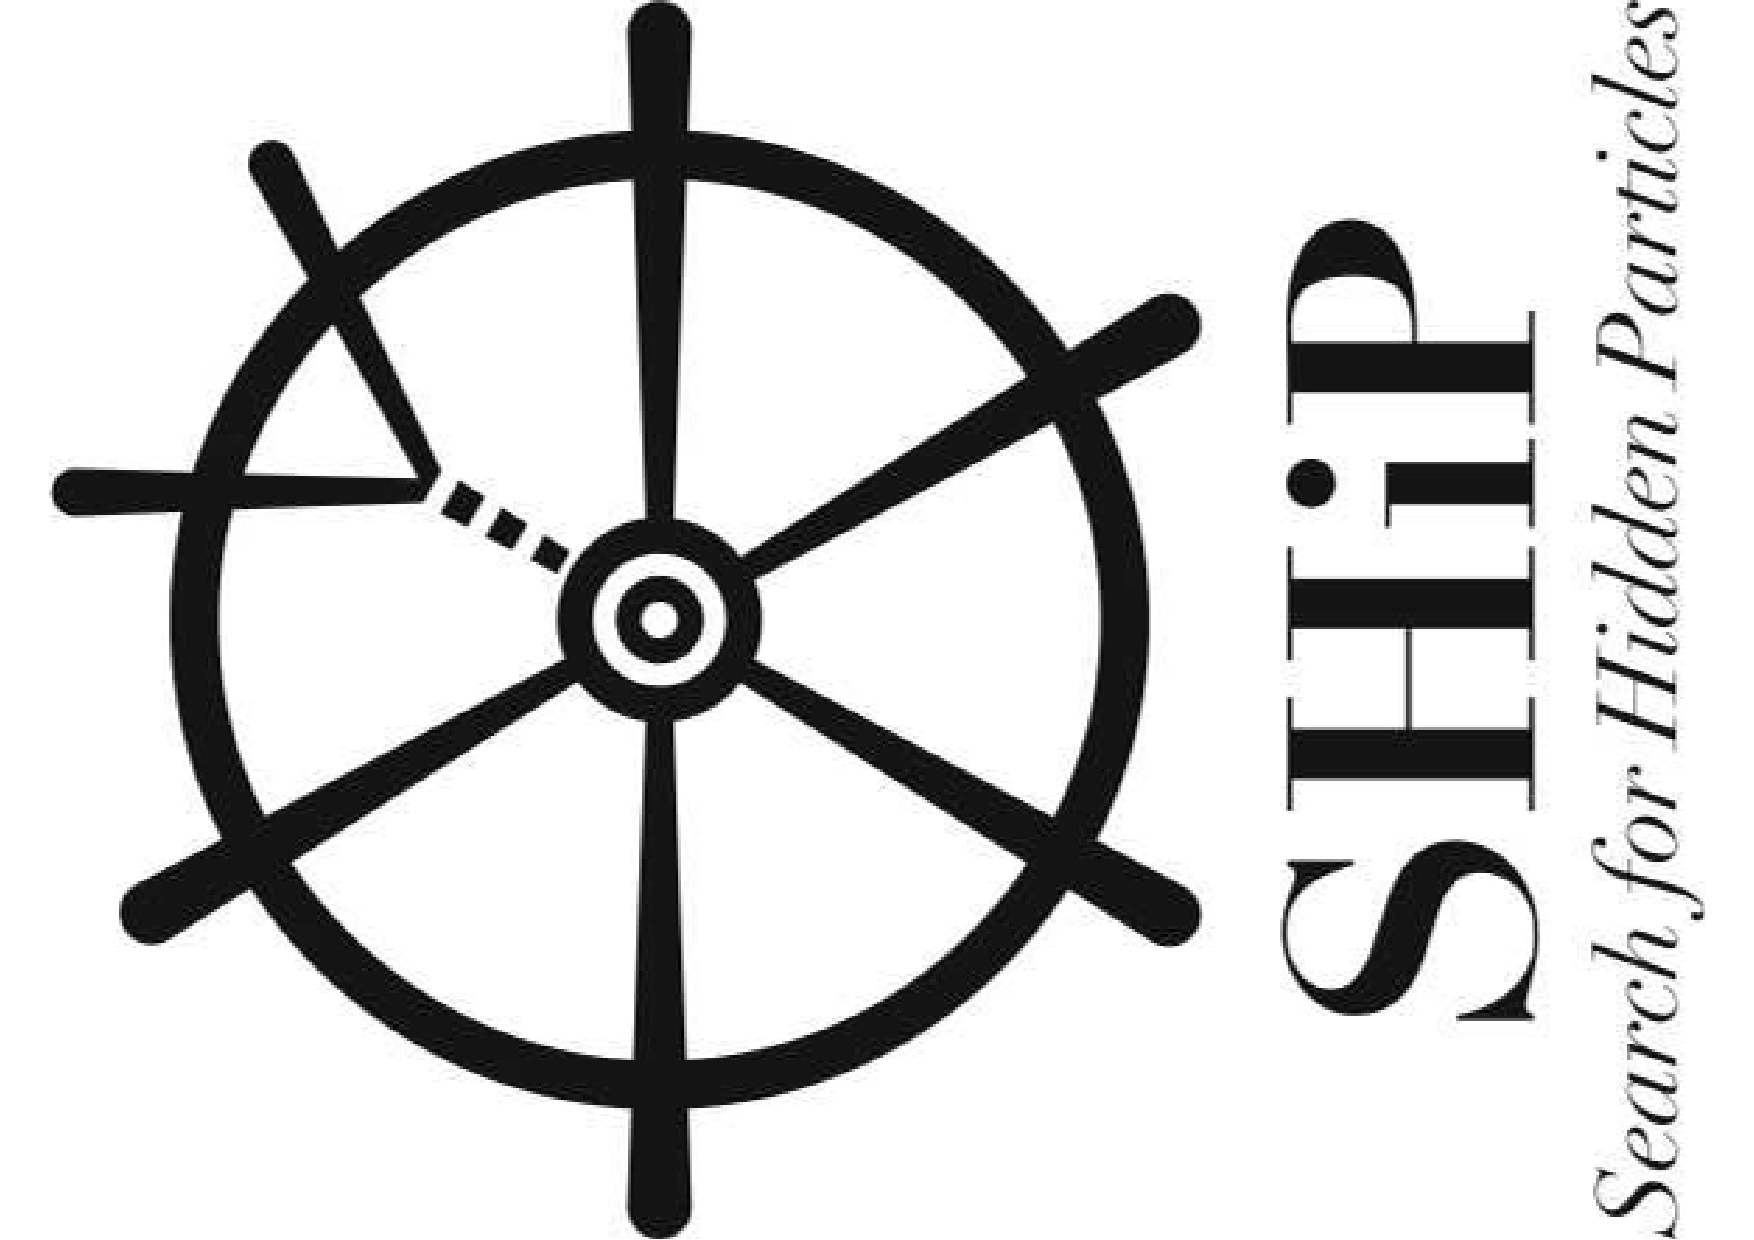
\includegraphics[angle=-90,width=0.15\textwidth,clip=]{SHiP-logo.pdf}}& & \\
&& SHiP-Note-2015-00X\\
&& 10 April 2015\\
\end{tabular*}
\vspace*{0.5cm}
\begin{center}
{\bf\huge\boldmath FairShip Manual \\}
\vspace*{0.9cm}
\end{center}
\vspace{\fill}

\large{M.~Frank$^{1}$, E.~Graverini$^{2}$, F.~Rademaker$^{3}$, T.~Ruf$^{3}$ and many others}\\
{$^{1}$\small\it CERN, Geneva, Switzerland}\\
{$^{2}$\small\it Physik-Institut, Universit\"at Zurich, Z\"urich, Switzerland}\\
{$^{3}$\small\it Humboldt-Universit\"at zu Berlin, Berlin, Germany}\\

\centerline{\bf Abstract}
\vspace*{3mm}\noindent  {\small 
An attempt to summarize the functionality and usage of \textsc{FairShip}.}
\vspace{\fill}

\end{titlepage}

%-------------------------------------------------------------------------\"
%     Table of Contents / List of Tables / List of Figures
%-------------------------------------------------------------------------
\tableofcontents
\newpage

%-------------------------------------------------------------------------
%     Main Text
%-------------------------------------------------------------------------
\section{Introduction}
\label{sec:intro}
%
The overall simulation and reconstruction software called \textsc{FairShip} is based on the \textsc{FairRoot}~\cite{AlTurany:2012gc} package, a lightweight software framework based on ROOT~\cite{root}. This note describes the functionality and the usage of it. 

\section{Packaging and Installation}
\label{sec:Installation}
The complete SHiP offline computing environment consists of three packages:
\begin{itemize}
   \item FairSoft: all packages needed by FairRoot, like ROOT, Geant3, Geant4, Pythia8, GENIE, GENFIT, etc.
   \item FairRoot: the FairRoot framework proper.
   \item FairShip: the SHiP specific implementation of the FairRoot classes.
\end{itemize}
These three packages are maintained on GitHub~\cite{computing:github} and can be installed and run on all major Linux distributions and on OSX. While the \textsc{FairShip} package changes frequently, the other two packages are rather stable. The GIT site ("https://github.com/ShipSoft/FairShip") also contains instructions how to install the packages, which are repeated for convenience shortly here:
\begin{itemize}
 \item Step 1: Set several required shell variables, needed during the installation and running of the different software packages:
 \begin{itemize}
  \item export SHIPSOFT=~/ShipSoft
  \item export SIMPATH=\$SHIPSOFT/FairSoftInst
  \item export FAIRROOTPATH=\$SHIPSOFT/FairRootInst
  \item export FAIRSHIP=\$SHIPSOFT/FairShip
  \item export FAIRSHIPRUN=\$SHIPSOFT/FairShipRun
 \end{itemize}
 \item Step 2: Install FairSoft
 \begin{itemize}
 \item mkdir \$SHIPSOFT 
 \item cd \$SHIPSOFT 
 \item git clone -b dev https://github.com/ShipSoft/FairSoft.git
 \item cd FairSoft
 \item cat DEPENDENCIES
 \item \# Make sure all the required dependencies are installed
 \item \# On SLC6 do: export FC=gfortran
 \item ./configure.sh
 \item \# 1) gcc (on Linux) 5) Clang (on OSX)
 \item \# 3) Optimization
 \item \# 1) Yes (install Simulation)
 \item \# 2) Internet (install G4 files from internet)
 \item \# 1) Yes (install python bindings)
 \item \# path: \$SHIPSOFT/FairSoftInst [\$SIMPATH is set in script]
 \end{itemize}
 \item Step 3: Install FairRoot
 \begin{itemize}
 \item cd \$SHIPSOFT
 \item git clone -b dev https://github.com/ShipSoft/FairRoot.git
 \item cd FairRoot
 \item mkdir build
 \item cd build
 \item cmake .. -DCMAKE\_INSTALL\_PREFIX=\$FAIRROOTPATH -DCMAKE\_BUILD\_TYPE=RELEASE
 (  on some platforms eventually use: 
 \item cmake .. -DCMAKE\_INSTALL\_PREFIX=\$FAIRROOTPATH -DCMAKE\_BUILD\_TYPE=RELEASE -DUSE\_DIFFERENT\_COMPILER=TRUE)
 \item make
 \item make install
 \item cd \$SHIPSOFT/FairRoot/build
 \item make test
 \end{itemize}
\item Step 4: Install the SHIP software:
\begin{itemize}
 \item cd \$SHIPSOFT (or at any other place XXX, assuming environment variable FAIRSHIP set to XXX/FairShip
 \item git clone https://github.com/ShipSoft/FairShip.git
 \item mkdir FairShipRun
 \item cd FairShipRun
 \item cmake ../FairShip
 \item (  on some platforms eventually use:  cmake ../FairShip -DUSE\_DIFFERENT\_COMPILER=TRUE)
 \item make
 \item ./config.sh
 \end{itemize}
\end{itemize}

In order to update the local version of \textsc{FairShip}, do 
\begin{itemize}
 \item
 \begin{itemize}
  \item cd \$FAIRSHIP 
  \item git pull 
 \end{itemize}
\end{itemize}

\section{Structure of FairShip}
\subsection{Folder /macro}
This is the directory for the steering macros, simulation, reconstruction and analysis. 

\subsection{Folder /python}
This is the directory for configuring the C++ objects. Also contains some useful python macros, for example shipunit.py, rootUtils.py. 

\subsection{Folder /shipgen}
Generators integrated into \textsc{FairShip} are located in the shipgen directory.
\begin{itemize}
\item  HNLPythia8Generator:  The generator for HNL signal events. It uses PYTHIA v8~\cite{pythia8} for the initial proton fixed target interaction. 
In all leptonic and semi-leptonic decay modes of charm particles, the neutrinos have been replaced by a HNL particle, with its
mass, lifetime and decay channels. Based on the mass of the HNL particle and its couplings, all possible decay modes with their
corresponding amplitudes are calculated and used to determine the lifetime of the HNL. Pions, kaons and other long-lived particles are set to stable. 
See also python/pythia8\_conf.py, python/DecaySelection.conf. Only the HNL decay products are given to GEANT4~\cite{Agostinelli:2002hh} for further processing.  

\item  GenieGenerator:     Reads inelastic neutrino interaction events produced by the GENIE~\cite{genie} generator for further processing inside SHiP.  
\item  MuonBackGenerator:  Reads in muons escaping the primary target and hadron absorber.
\item  MuDISGenerator:     Reads inelastic muon interaction events produced by the PYTHIA6~\cite{pythia6} generator for further processing inside SHiP.  
\item  CosmicsGenerator:
\end{itemize}

\subsection{Folder /muonShieldOptimization}
This is the directory for simulation and analysis of muon background. Contains a standalone PYTHIA8/GEANT4 python script to generate proton collisions in realistic target setup followed by a hadron absorber. All stable products after the hadron absorber are stored in a simple ROOT Ntuple for further processing inside \textsc{FairShip}, see MuonBackGenerator.
 

\subsection{Folder /geometry}
This directory contains files with geometry information, either in form of ascii files (for ECAL and HCAL) or encoded using python which allows more flexibility. 
\subsection{Folder /gconfig}
Configuration files for GEANT4 either plain ascii files or .C macros.

\subsection{Folder /passive}
This directory contains passive materials, like the target area, active and passive muon shield, spectrometer magnet, ...

\subsection{Folder /nutaudet}
This is the directory for the $\nu_\tau$ detector setup.

\subsection{Folder /veto}
This directory contains mainly the description of the decay vessel, together with the sensitive part liquid scintillator. But also, the 
upstream Veto tagger and the downstream timing detector, and a scoring plane further downstream at a place of a possible second detector.

\subsection{Folder /strawtubes}
This directory contains the description of the strawtube tracking detectors, including the  strawtube veto detector.

\subsection{Folder /field}
Analytic fieldmap for the SHiP spectrometer dipole magnet.

\subsection{Folder /ECAL}
\subsection{Folder /HCAL}
\subsection{Folder /Muon}

\subsection{Folder /genfit}
The package for track fitting installed from "http://genfit.sourceforge.net/Main.html"~\cite{Höppner2010518}. Note, it takes the geometry (material distribution) from importing the geofile saved during the MC simulation step. The magnetic field of the spectrometer, /field/ShipBellField.cxx, is implemented in genfit by genfit/fields/src/BellField.cc. 

\subsection{Folder /vm and /diag}
Related to virtual machine using docker.

\section{MC Event Generation, ShipSim}
Several use case are implemented in a Python script called ShipSim (previously called run\_simScript) described below. The output of these simulations are root files containing the produced Monte Carlo particles and the hits recorded in the sensitive detector parts. A cut is set at $>100\mev$ of kinetic energy to reduce the output data size ({\it fStack.SetEnergyCut(100.*u.MeV)}). A root file containing the full description of the geometry for further reconstruction is also being saved. With the --display option, the trajectories of the MC particles are stored for the event display. 

By default, the macro produces $100$ events of HNL signal type. In addition, the following options are available:

\begin{itemize}
\item -Y \textless height\textgreater : height of SHiP detector setup in $[m]$, default is $10$. 
\item --output, -o: output directory, default "."
\item --Pythia8 : default simulation engine, produce HNL signal events.
\item --mass, -m: mass of HNL in $[GeV/c^2]$, only valid for default simulation engine.
\item --couplings, -c: to set list of HNL couplings $U^2_e$, $U^2_\mu$, $U^2_\tau$.
\item --MuonBack : use muon background simulation engine.
\item --MuDIS: use muon inelastic scattering background engine.
\item --Genie : use neutrino background simulation engine.
\item --Cosmics: use Cosmics background simulation engine.
\item --nEvents, -n \textless N\textgreater: number of events to simulate.
\item -f \textless name\textgreater : path (if not in current directory) and name of inputfile, required for some background simulation engines.
\item --firstEvent, -i \textless N\textgreater: first event of input file to start simulation.
\item  --seed, -s \textless N\textgreater: seed for random number generator, if ommitted, constructed from current time.
\item --display, -D: default false, if set, additional information is stored of the trajectory of MC tracks.
\item --phiRandom: default false, if used, randomizes azimuth angle of incoming muons, used by muon background simulation engine.
\item --Pythia6: example of using Pythia6.
\item --NuRadio: abusing the neutrino background simulation engine to get a $\nu$-tomography of the material distribution.
\item --FollowMuon: default false, if set, only muons are followed in Geant4.
\item -F: default false, if set, all particles of a Pythia8 event are copied to FairShip processing.
\item -A: default false, if set, Pythia8 is configured for minimum bias events.
\item --Ntuple: example of simulation engine reading events from input file.
\end{itemize}

\subsection{Signal (HNL) Generation}
Command: python \$FAIRSHIP/macro/ShipSim.py -n (number of events) --mass (mass of HNL) --couplings \'U2e,U2mu,U2tau\'. The default settings are for $M=1\gevcc$ and couplings corresponding to a mean decay length of $54\,$km. 
 
\subsection{Muon background originating from primary target}
Command: python \$FAIRSHIP/macro/ShipSim.py -n (number of events) -i (first event) --MuonBack -f (input file). Muons escaping the hadron absorber close to the primary target are read from an external file (pythia8\_Geant4\_Yandex\_onlyMuons.root, pythia8\_Geant4\_onlyMuons.root,  pythia8\_Geant4\_MoTarget\_234M\_onlyMuons.root), propagated through the muon shield and the detector setup. The -i option is useful if the processing is done with the same input file over many cores in parallel.

\subsection{Neutrino induced background}
Command: python \$FAIRSHIP/macro/ShipSim.py -n (number of events) -i (first event) --Genie -f (input file). Template events for neutrino inelastic scattering produced by the GENIE generator are read in and distributed along the flight path of these neutrinos taking into account the material distribution. 

\subsection{Muon induced background}
Command: python \$FAIRSHIP/macro/ShipSim.py -n (number of events) -i (first event) --MuDIS -f (input file). Template events for muon inelastic scattering produced by the PYTHIA6 generator are read in and distributed along the flight path of these muons taking into account the material distribution. 

\subsection{Cosmic muon background}

\section{Configuration}
\subsection{Geometry}
Basic geometry parameters are encoded in the file geometry/geometry\_config.py, except for ECAL and HCAL, which use plain ascii files (ecal\_ellipse5x10m2.geo and hcal.geo). Using python as programming language makes it easy to configure the setup for different geometry layouts and detector options. The configuration of the C++ objects is done inside macro/shipDet\_conf.py, importing the basic constants from geometry/geometry\_config.py. 

The version of the Geant4 Virtual Monte Carlo v2-15a does not support the setting of constant magnetic fields inside volumes. A workaround is provided with   
python/geomGeant4.py, which takes the field value of the TGEO objects and copies it to the corresponding Geant4 volumes.    
 
\subsection{Particle Generators}
The configuration of Pythia8 for different use cases is done with pythia8\_conf.py. The decay properties of the HNL particle is derived from its hypothetical mass and coupling constants, hnl.py.

\section{Reconstruction, ShipRec}
The reconstruction steps are performed using macro/ShipRec.py. This includes so far digitization of strawtube hits, fake pattern recognition to form track candidates, track fitting using GENFIT and ECAL cluster reconstruction. The macro can be called with the following options:

\begin{itemize}
\item --inputfile=, -f \textless name\textgreater : path (if not in current directory) and name of inputfile.
\item --geoFile=,   -g \textless name\textgreater : path (if not in current directory) and name of geofile. If ommitted, try to guess name from inputfile.
\item -Y \textless height\textgreater             : height of SHiP detector setup in $[m]$, if ommitted guessed from inputfile name. 
\item --nEvents=, -n  \textless N\textgreater      : number of events to process, if ommitted, process all events.
\item saveDISK:  default false, if option specified, inputfile will be removed. All data copied in any case to output file.
\item noStrawSmearing:  default on, if option specified, no smearing of distance to wire. 
\item EcalDebugDraw:  default false, for debugging ECAL cluster reconstruction. 
\end{itemize}
The name of the output file is made using from the name of the input file and adding "\_rec". 


\subsection{Strawtube measurements}
Each strawtube MC hit is converted into a measurement consisting of the start and end points of the wire, and the distance to the wire which is randomly smeared within the expected detector resolution. This information is made persistent in the SmearedHits branch of the output tree.  
\subsection{Fake pattern recognition}
While a pattern recognition without using MC truth is still under development, a fake pattern recognition is put in place which sorts all strawtube measurements according to the particle which produced the MC hit. A hit list with more than 24 entries and hits in at least 3 tracking stations is used as input for the track fit. The navigation back to the MC truth is provided by the branch fitTrack2MC, which takes as input the index of the track candidate and returns the index of the underlying MCTrack.   

\subsection{Track fit}
The fitting of the track candidates is made with the genfit package using an Deterministic Annealing Filter (DAF). The DAF is an iterated Kalman filter, which has the advantage to solve the {\em top-bottom} ambiguities of the strawtube timing measurement. An initial state is made with an error in y and z of the expected detector resolution and an error in x (stereo) 10x larger. 

\subsection{Vertexing}
The point of closest approach between two tracks is determined in an iterative procedure. It starts with calculating the vertex using a linear track model. Knowing this intermediate vertex, the two tracks are extrapolated through the magnetic field using the extrapolator method of the genfit package. A new vertex is calculated using again a linear track model. If the distance between new vertex and old vertex is less than $1\,$mm, the procedure is stopped. The momentum of the two tracks at this positon is calculated and used to determine the momentum of a hypothetical particle decaying in two particles. The mass hypothesis for the two tracks is taken from the MC truth for (electrons, muons, pions) assuming sufficient good particle identification available using ECAL, HCAL and muon detectors, while for protons, the pion mass is used.    

\subsection{ECAL clustering}

\section{Analysis, ShipAna}
Mainly a template for starting to write a specific analysis program. Also useful for testing.  

\section{Event display, eventdisplay}
The eventdisplay is started with macro/eventdisplay.py. A basic .C version can also be found in macro/obsolete/eventdisplay.C.  


\bibliography{TP_SHiP}     
\bibliographystyle{SHiP}

\end{document}
